\section{Figures}



\begin{figure}
	\centering
		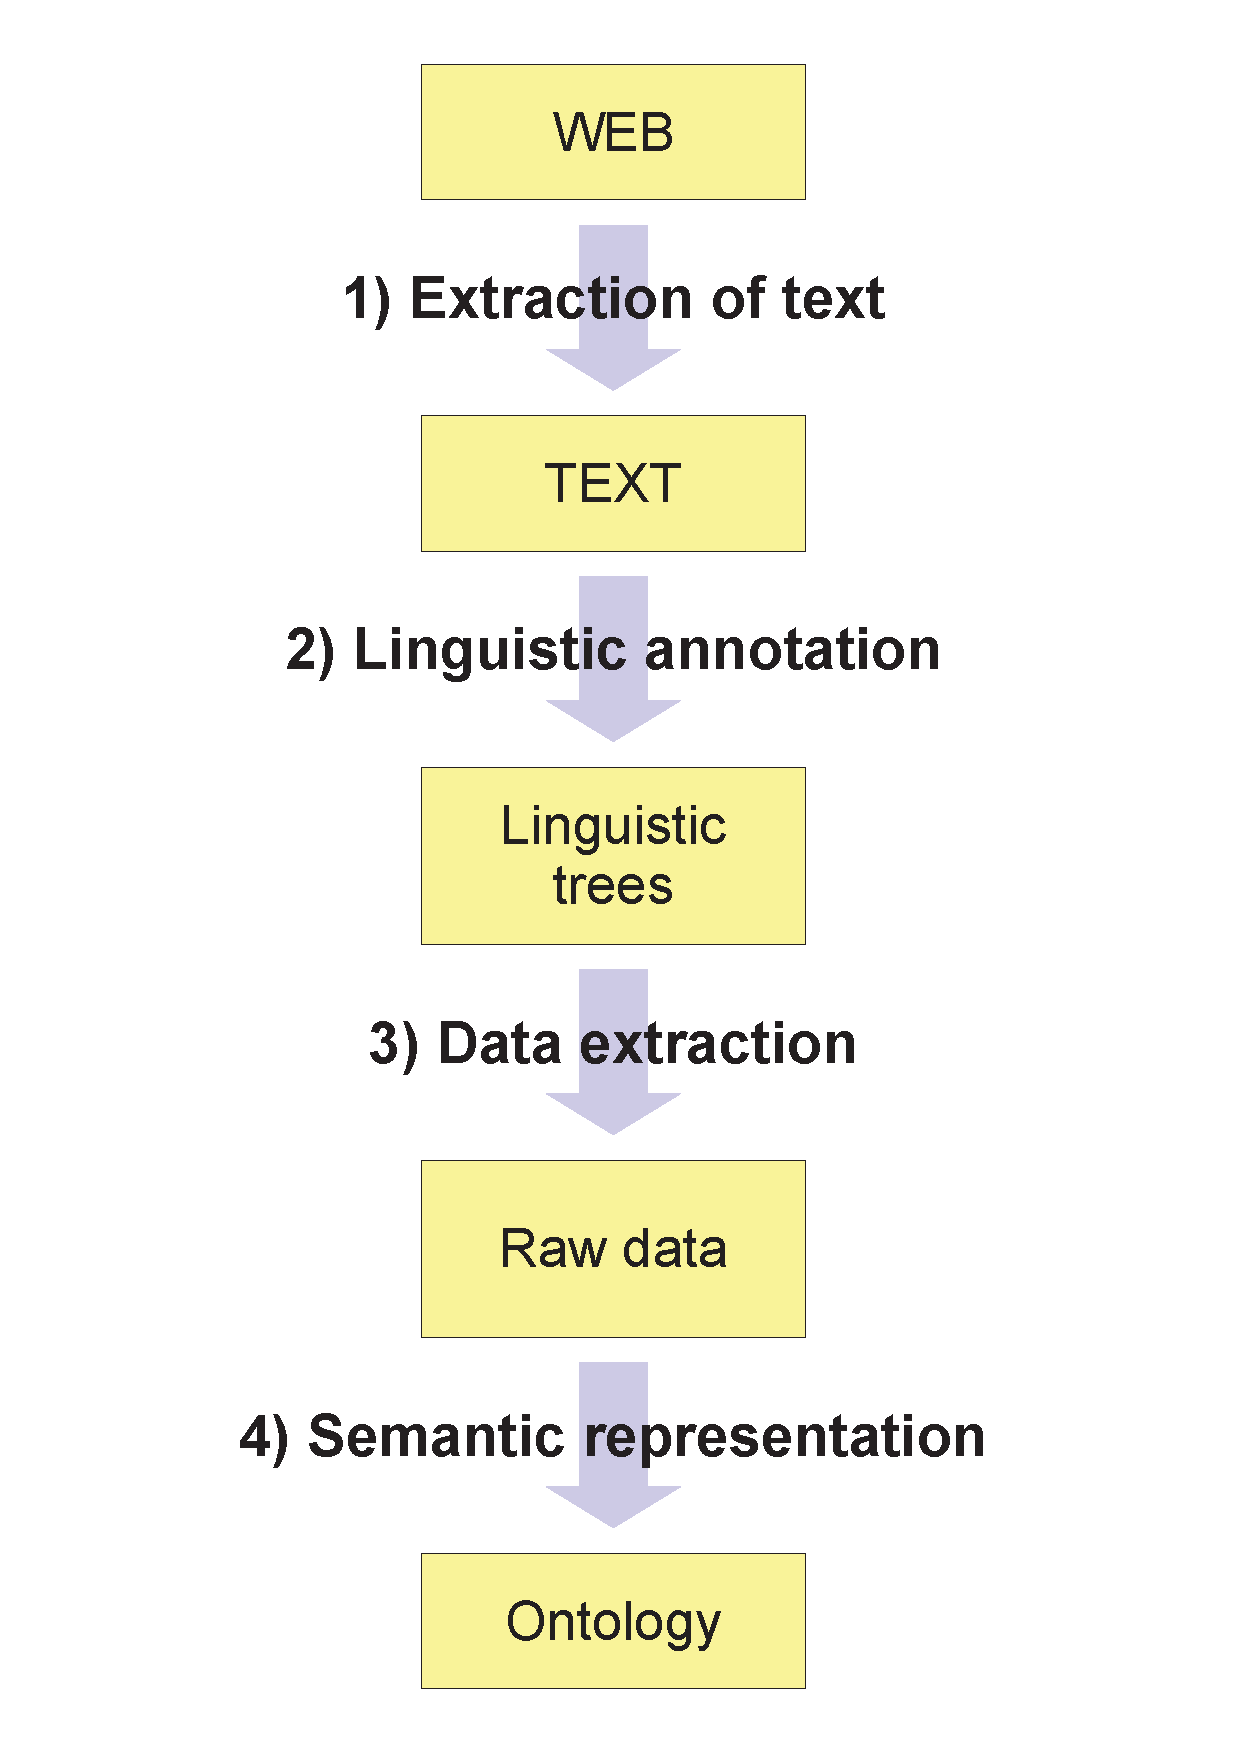
\includegraphics[width=0.2\hsize]{../img/ch3_ap_schema}
	\caption{Schema of the extraction process.}
	\label{fig:ch3_ap_schema}
\end{figure}


\begin{figure}
	\centering
		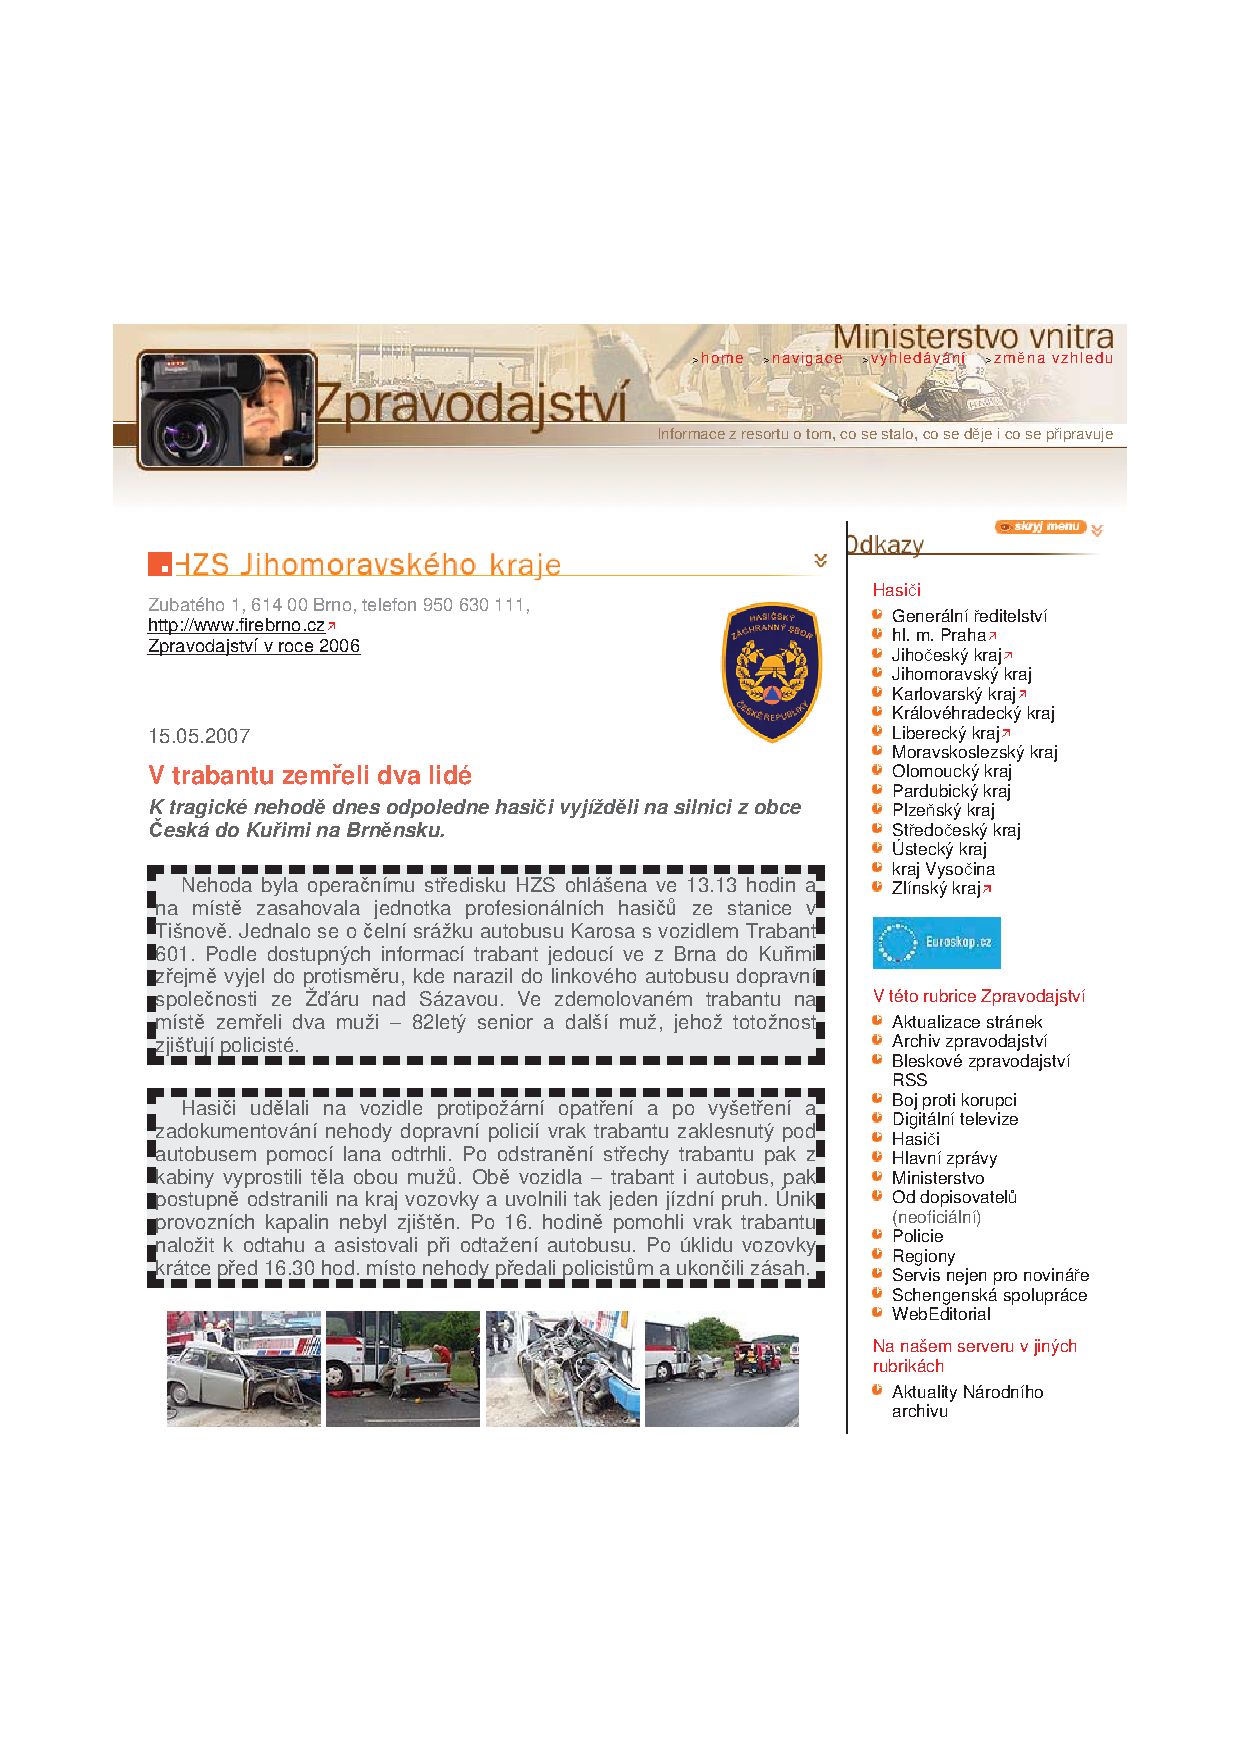
\includegraphics[width=0.5\hsize]{../img/ch3_article}
	\caption{One web page with an accident report.}
	\label{fig:ch3_article}
\end{figure}


\begin{figure}
	\centering
		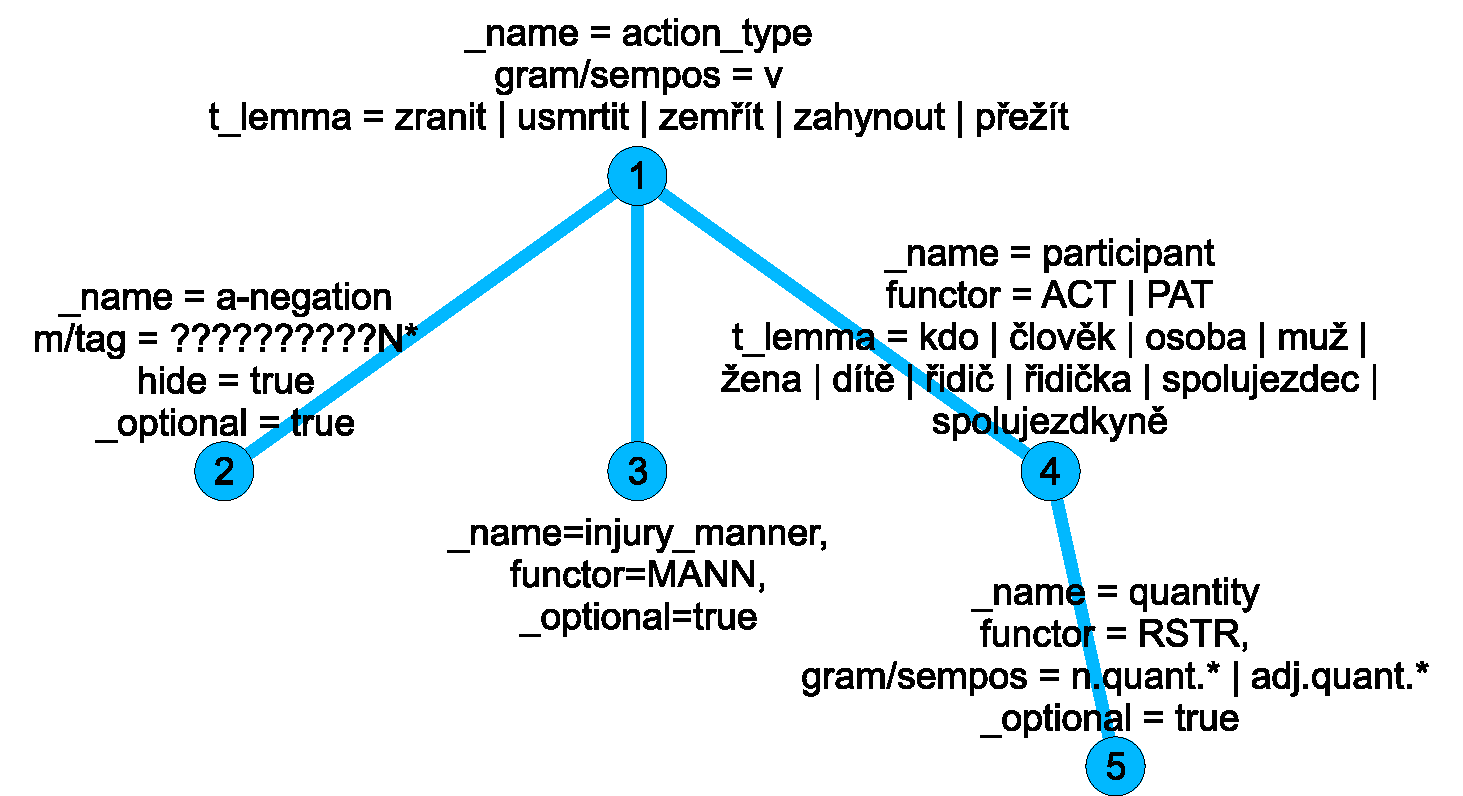
\includegraphics[width=0.5\hsize]{../img/ch3_extract_patern}		
\\Transcript:\\
\begin{tabular}{|c|c|c|c|c|}
\hline
zranit & usmrtit & zemřít & zahynout & přežít\\
to injure & to kill & to die & to wane & to survive\\
\hline
\end{tabular}
\\\begin{tabular}{|c|c|c|c|c|c|}
\hline
kdo & člověk & osoba & muž & žena & dítě\\
somebody & (hu)man & person & man & woman & child\\
\hline
\end{tabular}
\\\begin{tabular}{|c|c|c|c|}
\hline
řidič & řidička & spolujezdec & spolujezdkyně\\
driver & woman driver & passenger & woman passenger\\	
\hline
\end{tabular}		
	\caption{A manually created extraction rule investigating numbers of injuries and fatalities.}
	\label{fig:ch3_extract_patern}
\end{figure}

\begin{figure}
	\centering
		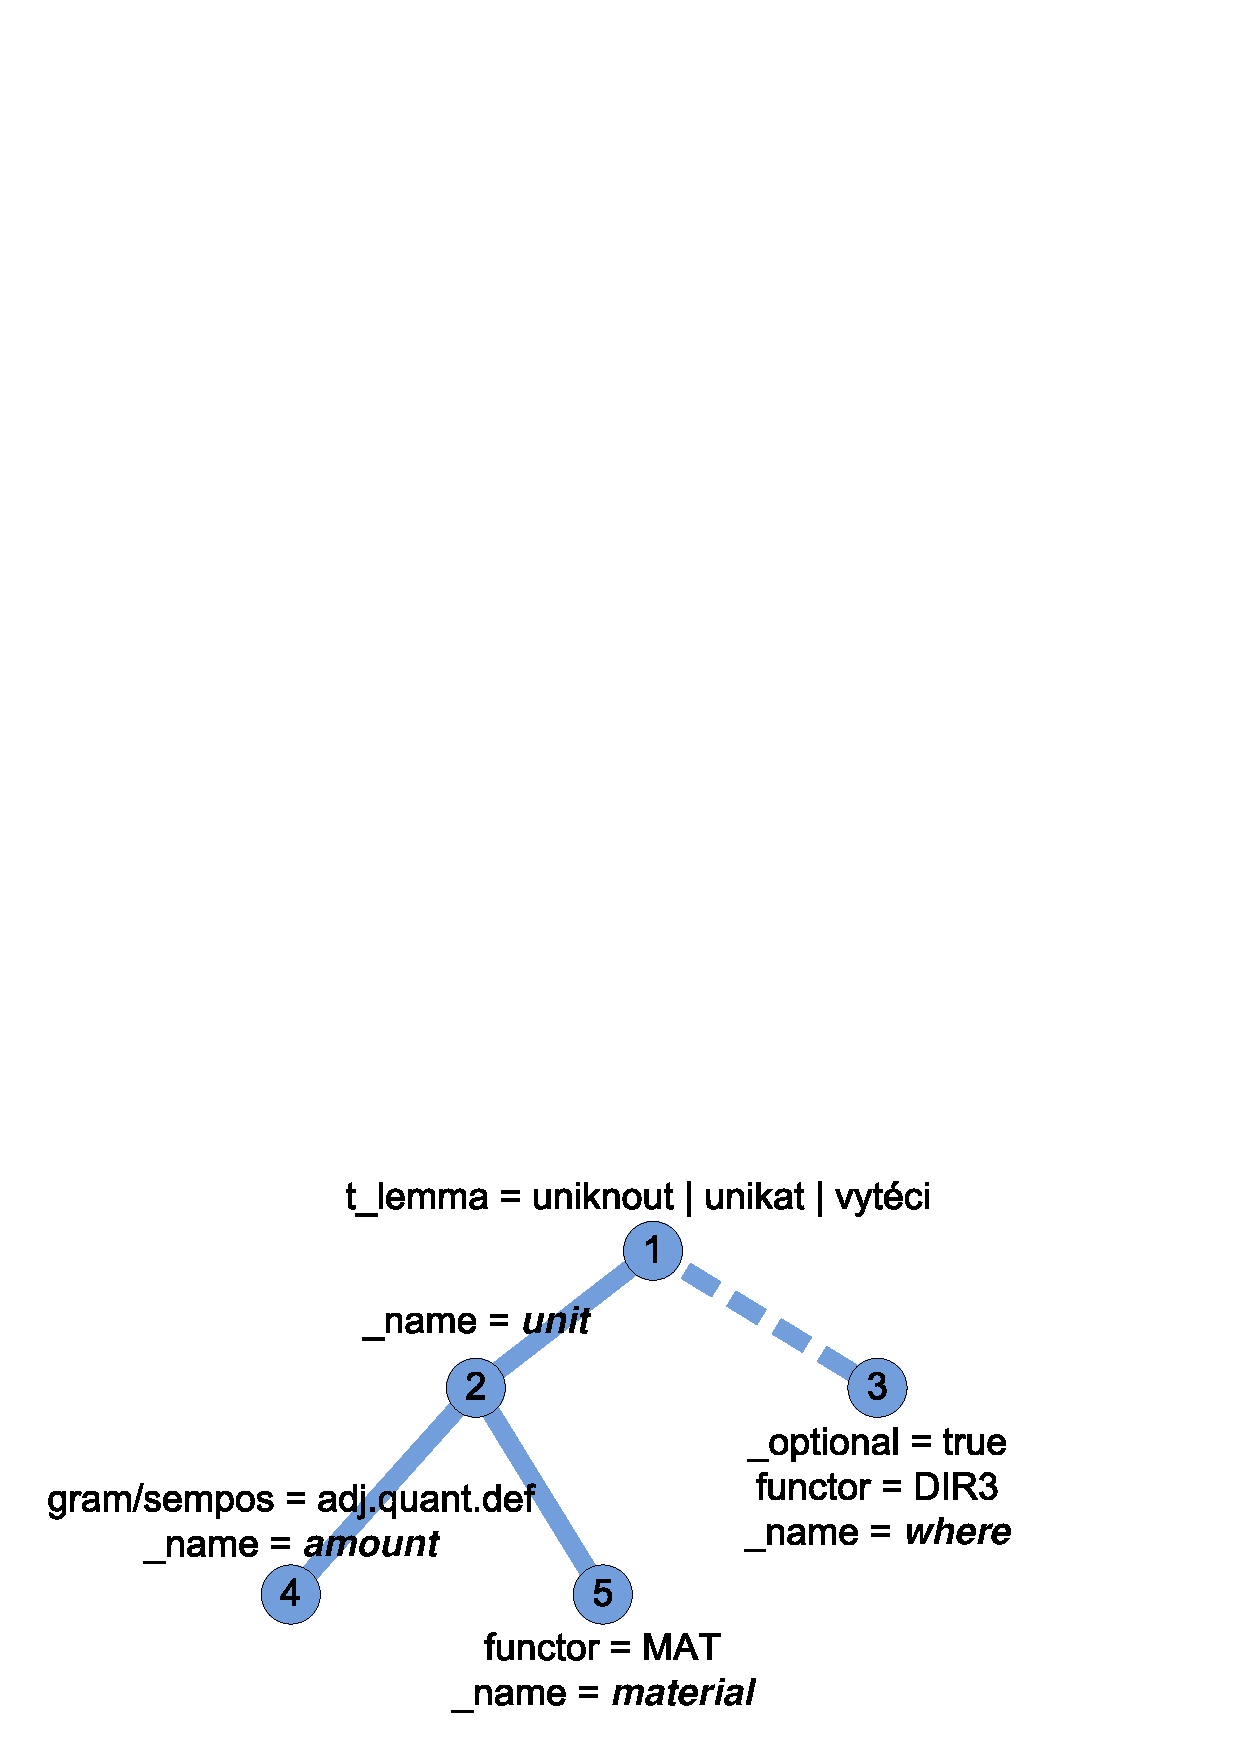
\includegraphics[width=0.5\hsize]{../img/ch3_eenv_extract_patern}
	\caption{A manually created extraction rule investigating dangerous liquids that spilled out into the environment.}
	\label{fig:ch3_eenv_extract_patern}
\end{figure}


\begin{figure}
	\centering
		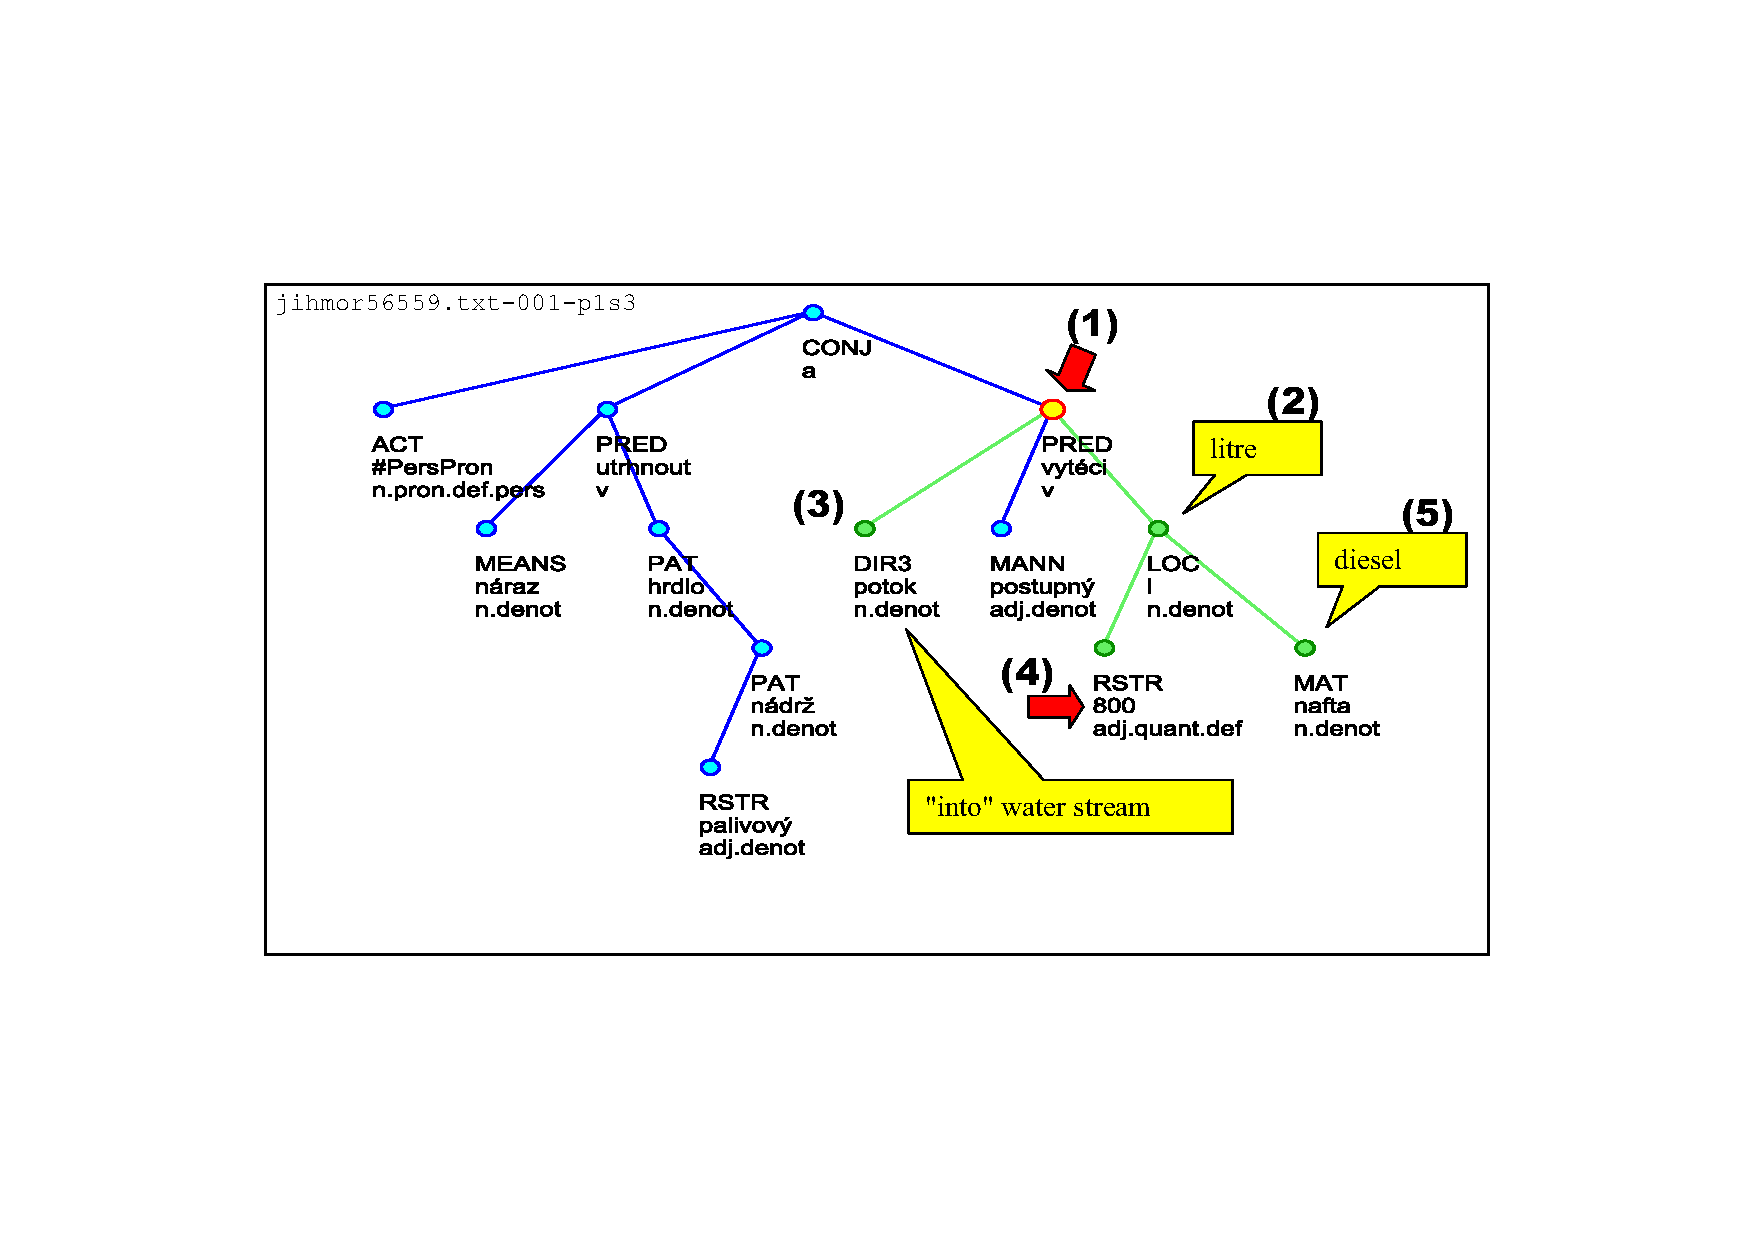
\includegraphics[angle=-90, width=0.6\hsize]{../img/ch3_eenv_matching_tree}
		
Original sentence: 
\emph{``Nárazem se utrhl hrdlo palivové nádrže a do potoka postupně vyteklo na 800 litrů nafty.''}\\
English transcript: 
\emph{``Due to the clash the throat of fuel tank tore off and 800 liters of oil (diesel) has run out to a stream.''}
	\caption{A tree matching with the corresponding extraction rule in Figure~\ref{fig:ch3_eenv_extract_patern}.}
	\label{fig:ch3_eenv_matching_tree}
\end{figure}


\begin{figure}
	\centering
		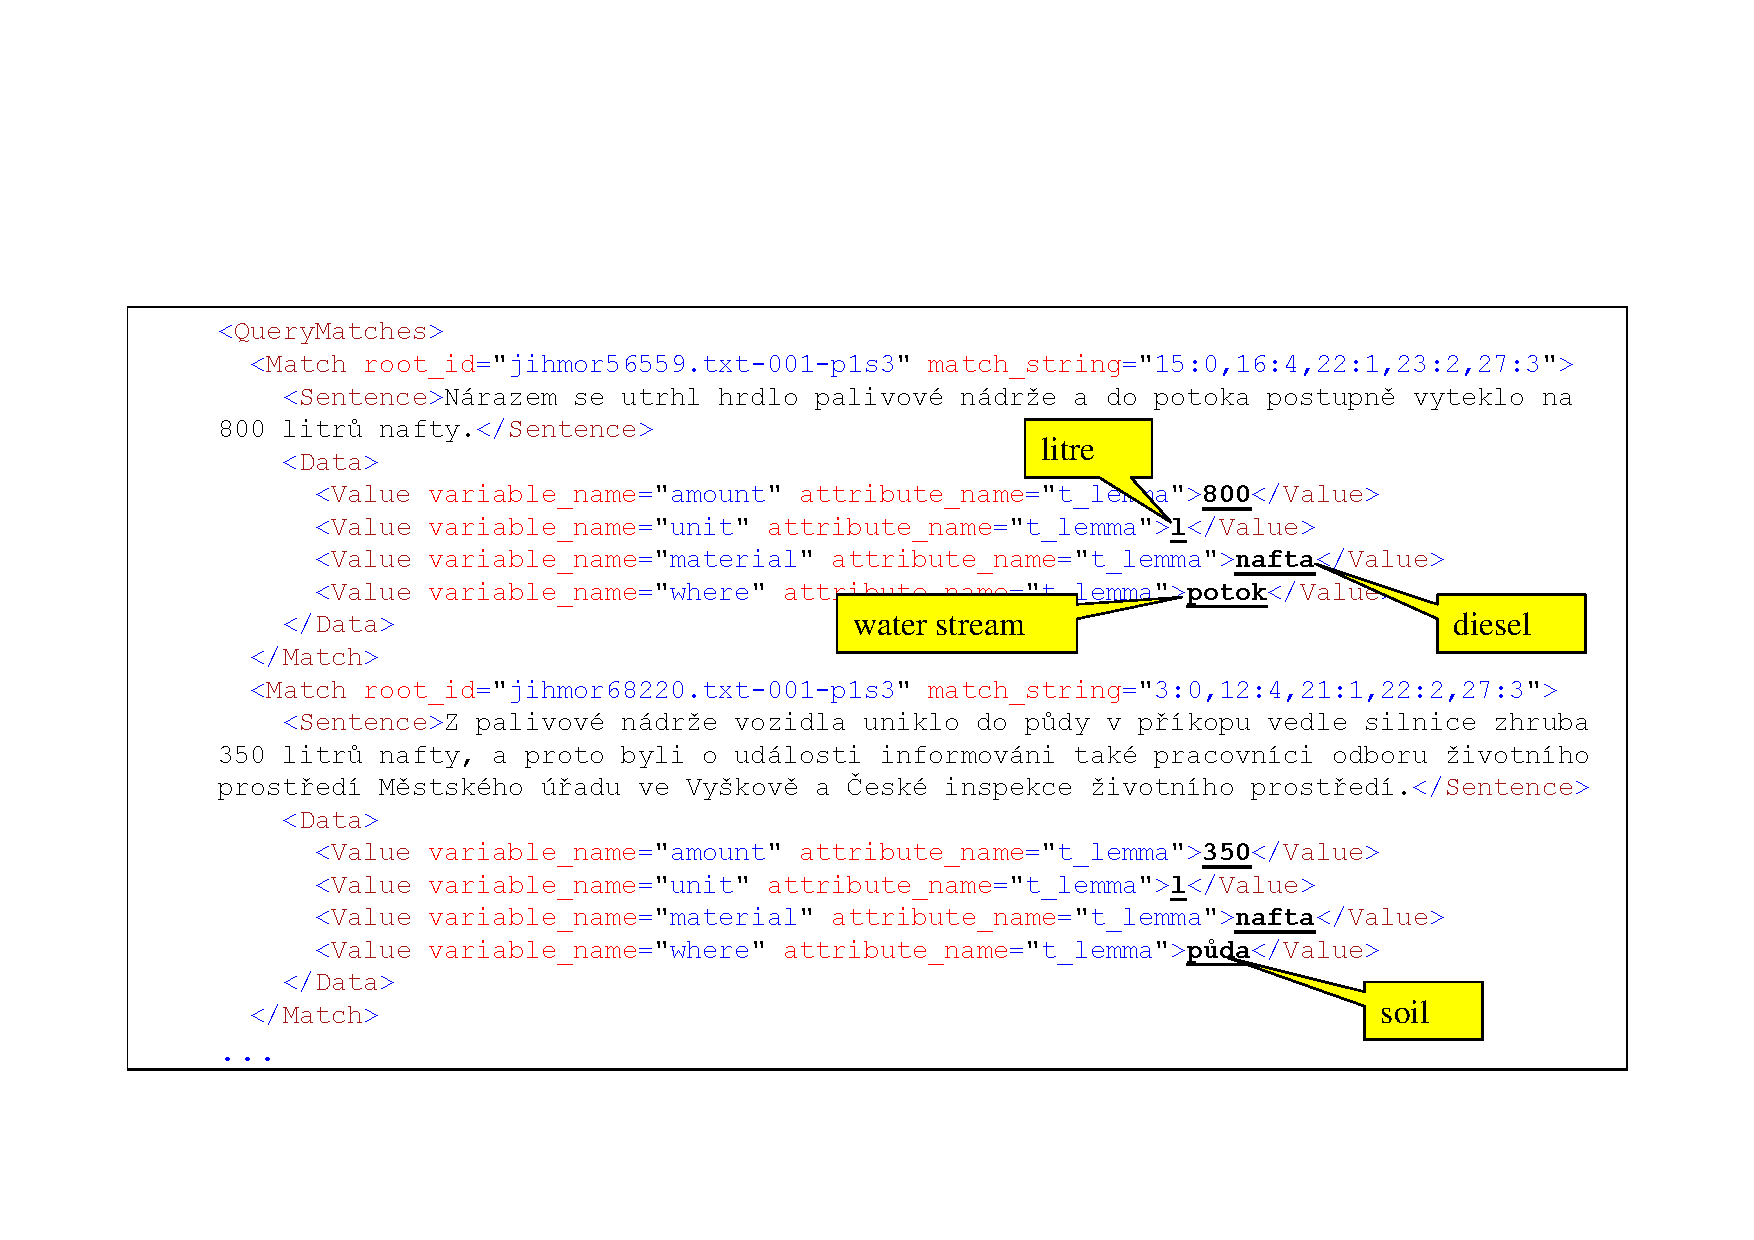
\includegraphics[angle=-90, width=0.7\hsize]{../img/ch3_eenv_results}
	\caption{\emph{XML} structured output of the SQL select like query corresponding with the extraction rule in Figure~\ref{fig:ch3_eenv_extract_patern} and matching tree in Figure~\ref{fig:ch3_eenv_matching_tree}.}
	\label{fig:ch3_eenv_results}
\end{figure}



\begin{figure}
	\centering
		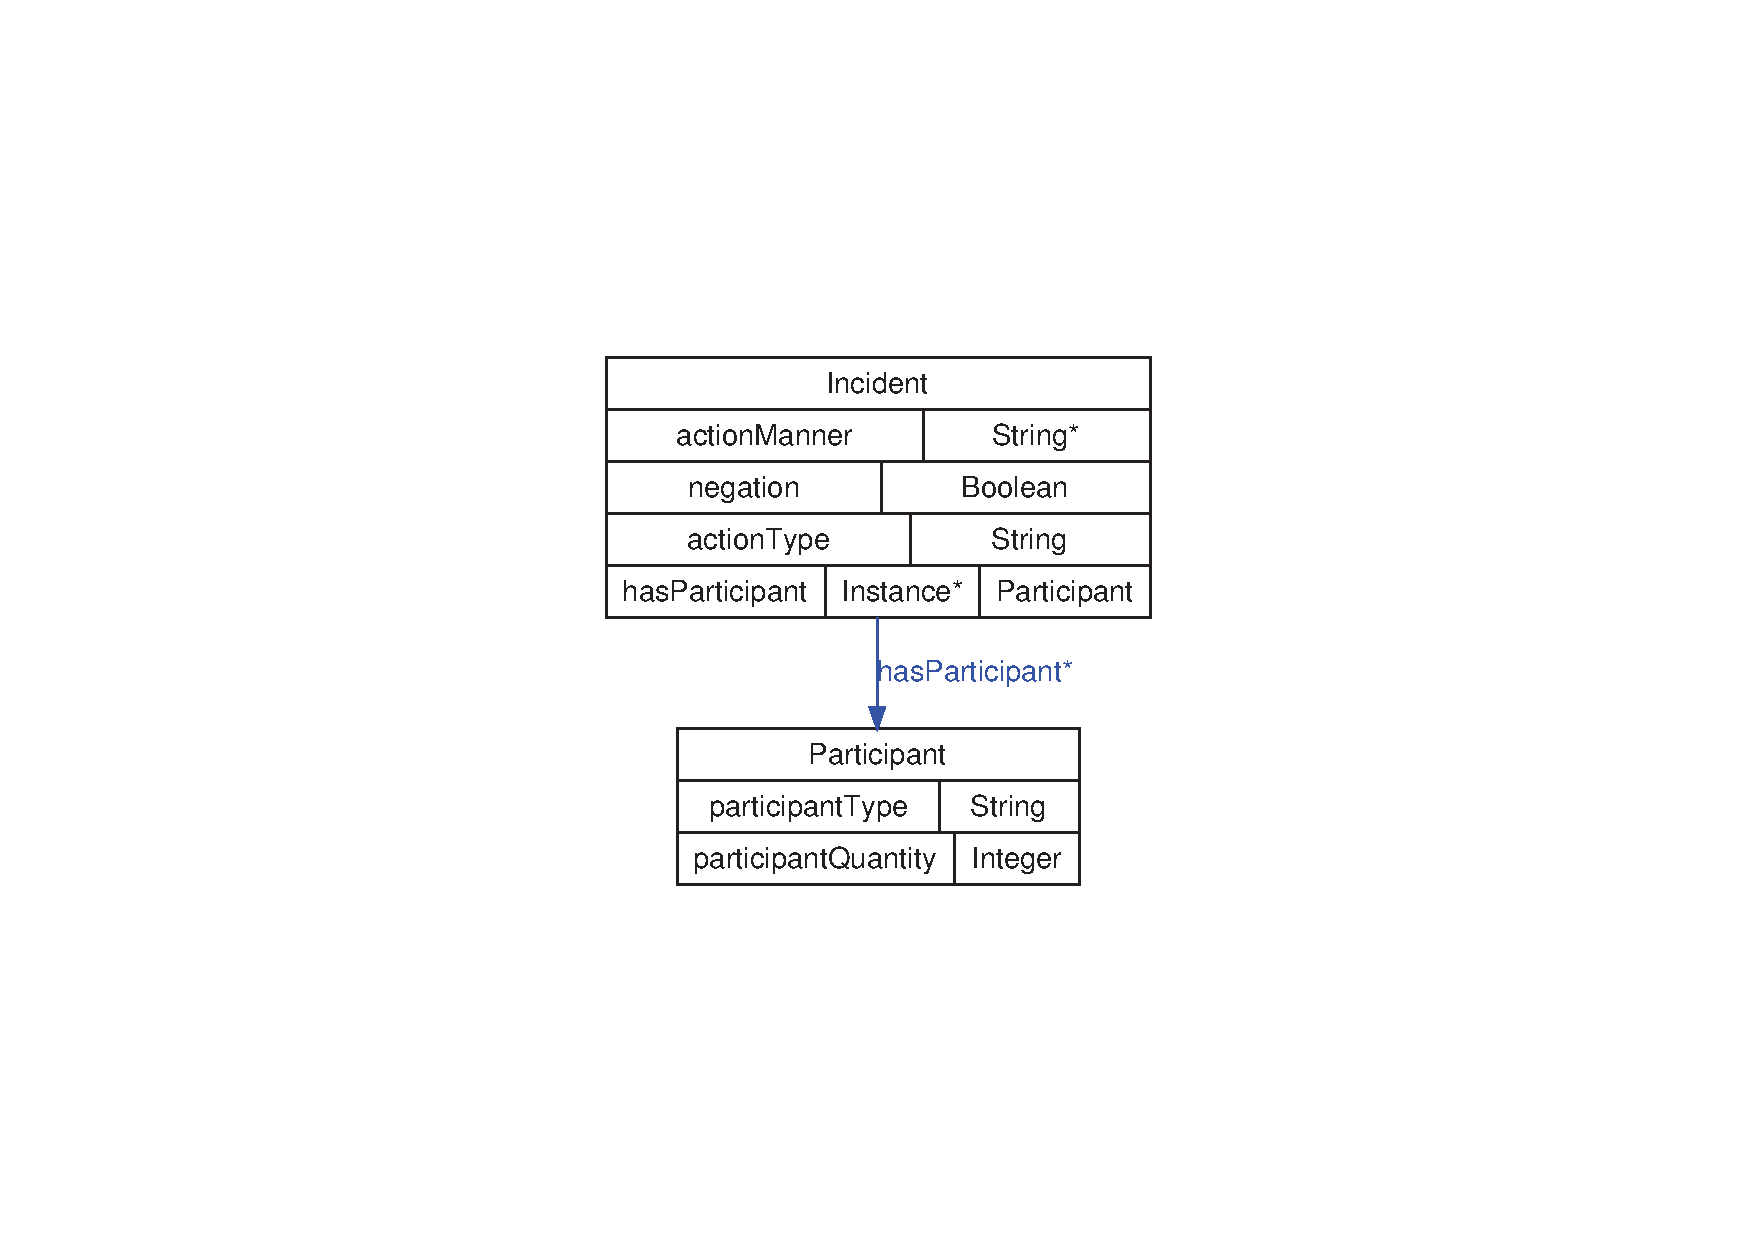
\includegraphics[angle=-90, width=0.3\hsize]{../img/ch3_classes}
	\caption{Schema of the target ontology.}
	\label{fig:ch3_classes}
\end{figure}


\begin{figure}
	\centering
		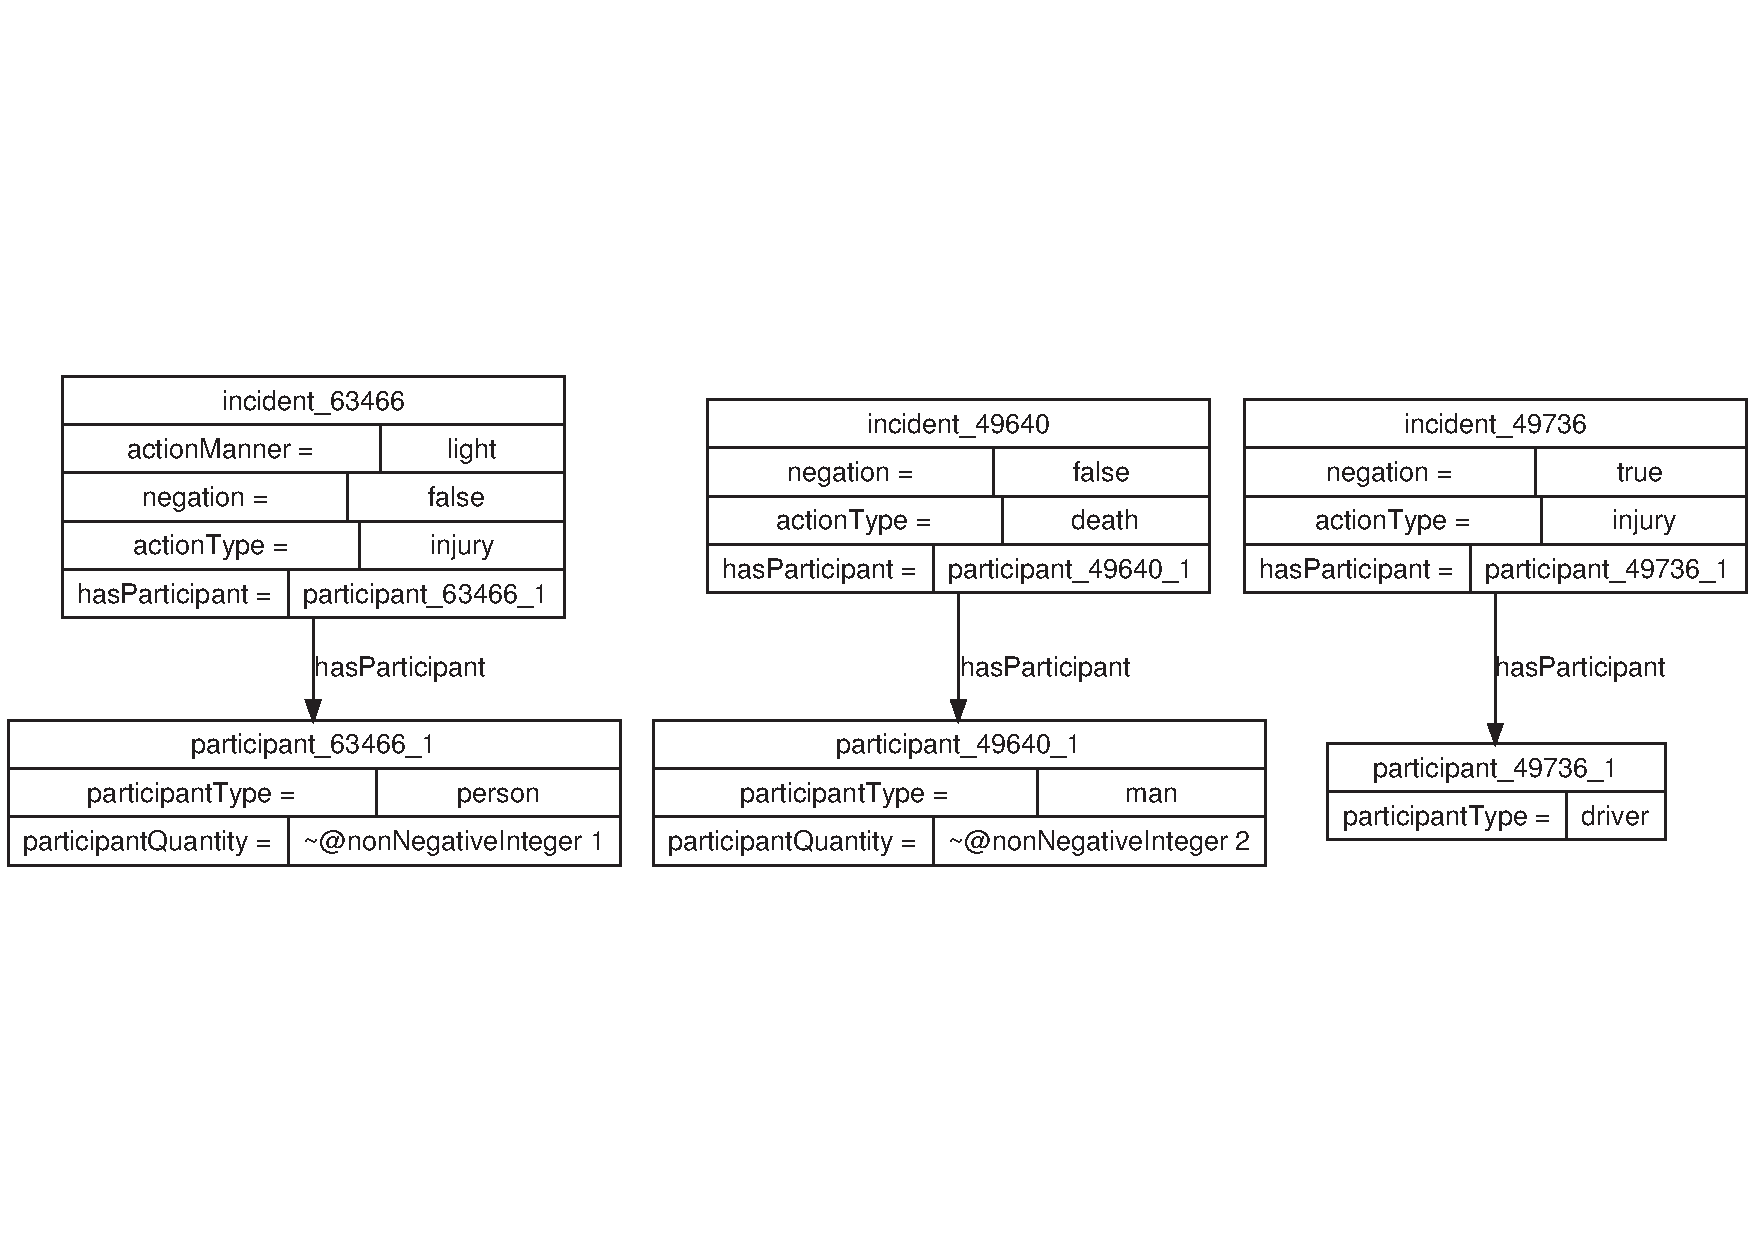
\includegraphics[angle=-90, width=\hsize]{../img/ch3_instances}
	\caption{Extracted instances of the target ontology.}
	\label{fig:instatnces}
\end{figure}


\begin{figure}
	\centering
		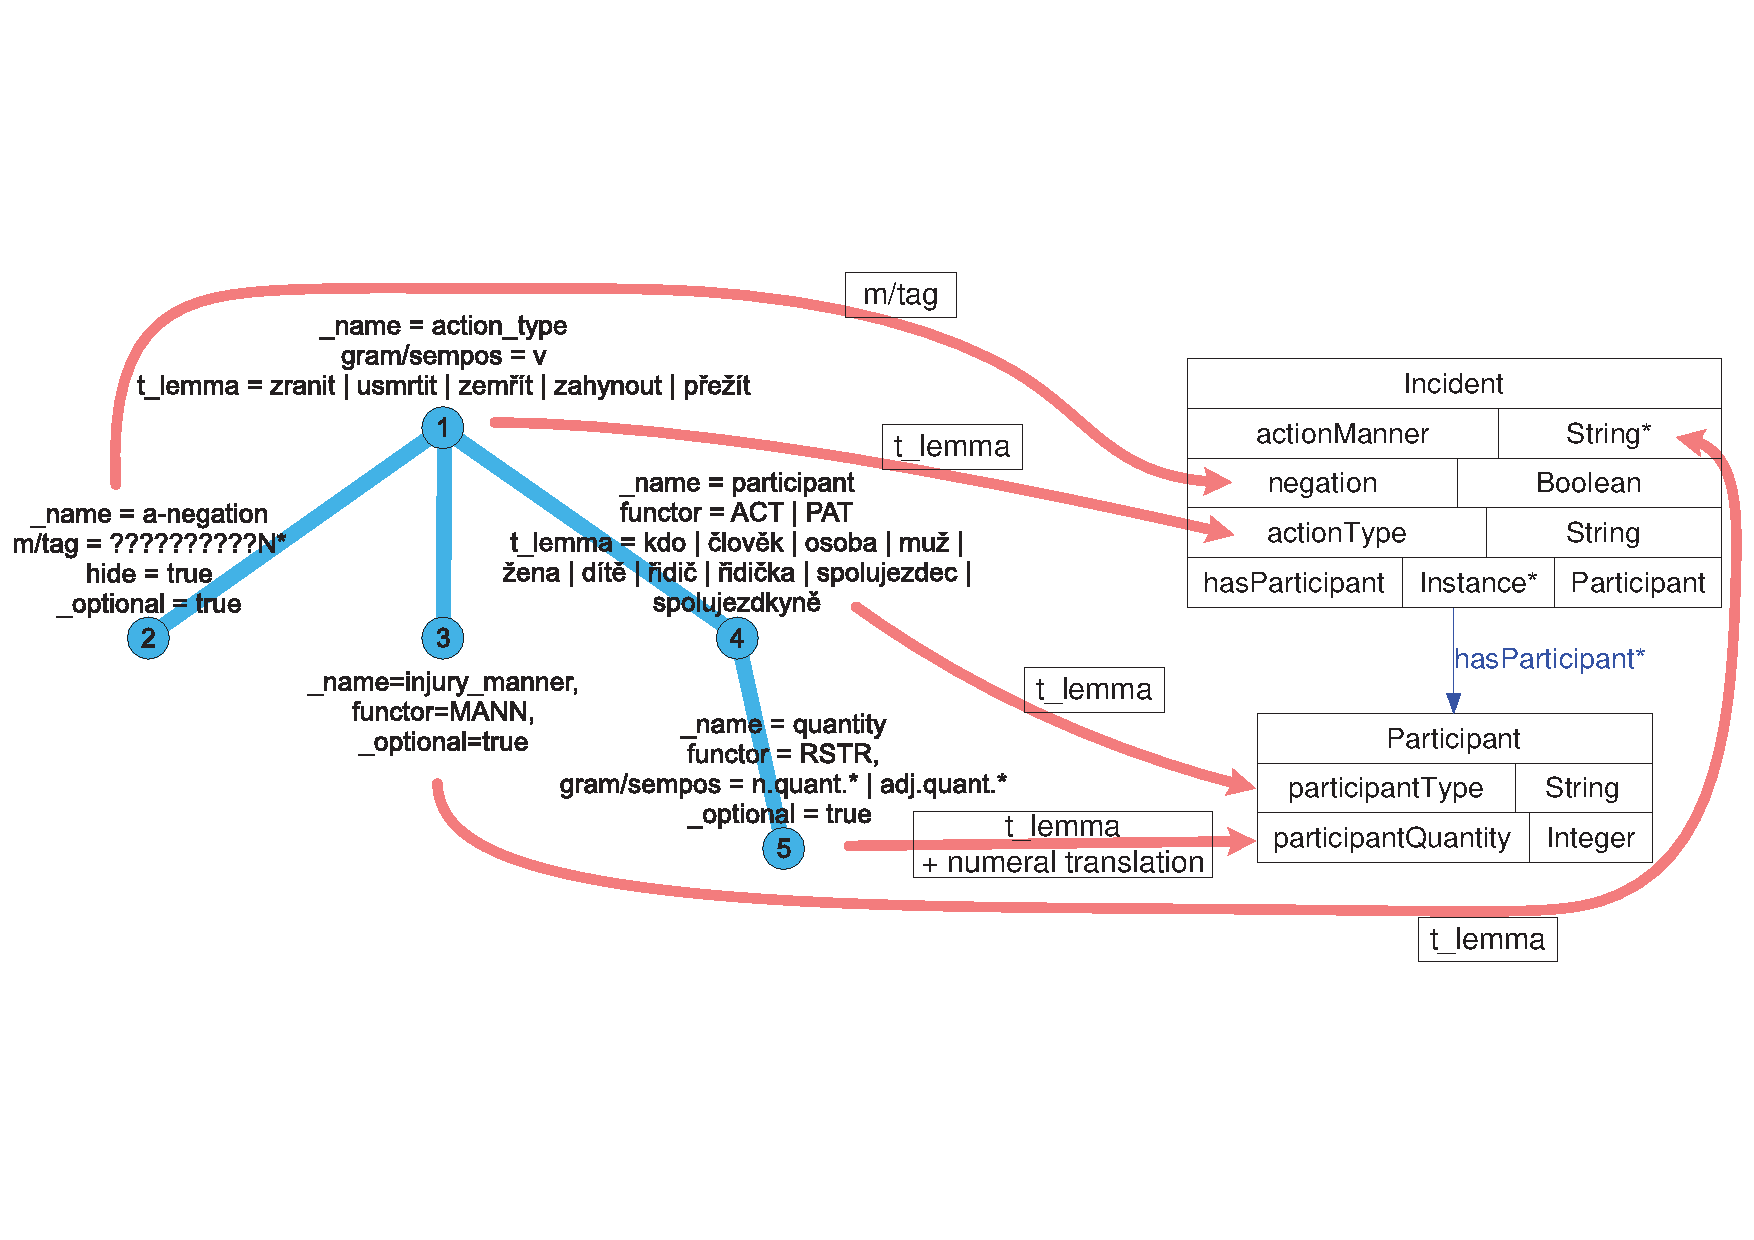
\includegraphics[angle=-90, width=0.9\hsize]{../img/ch3_semantic_interpretation}
	\caption{Semantic interpretation of the extraction rule.}
	\label{fig:ch3_semantic_interpretation}
\end{figure}


\begin{figure}
	\centering
		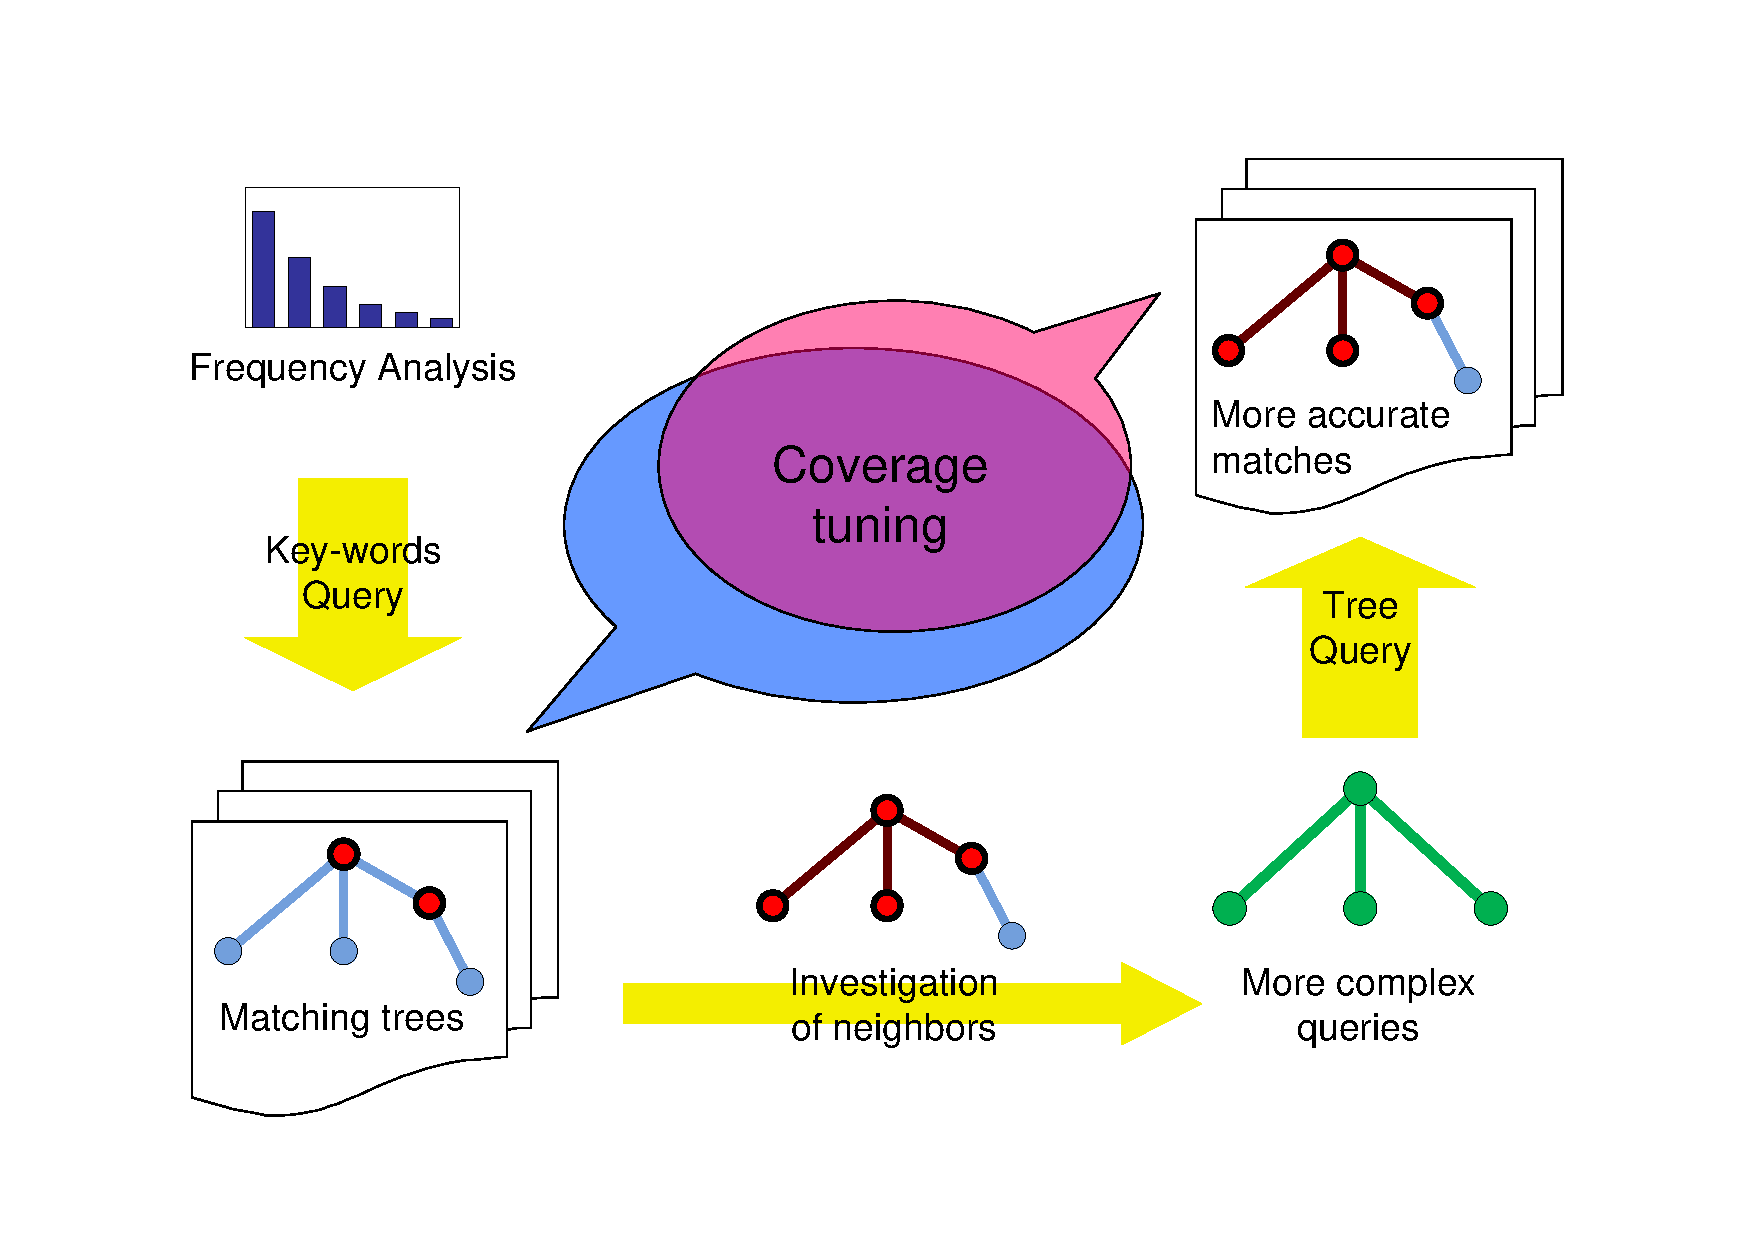
\includegraphics[angle=-90, width=0.5\hsize]{../img/ch3_coverge_tuning}
	\caption{Gradual refinement of an extraction rule.}
	\label{fig:ch3_coverge_tuning}
\end{figure}


\begin{figure}
\fbox{\parbox[b]{\hsize}{
\hspace*{0cm}$\bullet$ entita:1\\
\hspace*{1cm}$\bullet$ objekt:1\\
\hspace*{2cm}$\bullet$ celek:1\\
\hspace*{3cm}$\bullet$ artefakt:1, výtvor:2, výrobek:2\\
\hspace*{4cm}$\bullet$ vybavení:2\\
\hspace*{5cm}$\bullet$ přepravní prostředek:1, transportní prostředek:1\\
\hspace*{6cm}$\triangleright$ \textbf{veřejná doprava:1}\\
\hspace*{7cm}$\Rightarrow$ \emph{autobus:1, autokar:1}\\
\hspace*{6cm}$\triangleright$ \textbf{dopravní prostředek:1}\\
\hspace*{7cm}$\bullet$ kolové vozidlo:1\\
\hspace*{8cm}$\bullet$ samohybné vozidlo:1, vozidlo s vlastním pohonem:1\\
\hspace*{9cm}$\bullet$ motorové vozidlo:1\\
\hspace*{10cm}$\bullet$ nákladní automobil:1\\
\hspace*{11cm}$\Rightarrow$ \emph{kamion:1}

\vspace{1cm}

\setlength{\columnsep}{0cm}

\begin{multicols}{2}

\hspace*{0cm}$\bullet$ motorové vozidlo:1\\
\hspace*{1cm}$\bullet$ motocykl:1\\
\hspace*{1cm}$\bullet$ nákladní automobil:1\\
\hspace*{1cm}$\bullet$ obojživelné vozidlo:1\\
\hspace*{1cm}$\bullet$ auto:1, vůz:2\\
\hspace*{1cm}$\bullet$ pohřební vůz:1\\
\hspace*{1cm}$\bullet$ sněžný pluh:1, pluh:2\\
\hspace*{1cm}$\bullet$ golfový vozík:1\\

\vspace{0.5cm}

\hspace*{0cm}$\bullet$ nákladní automobil:1\\
\hspace*{1cm}$\bullet$ dodávka:3\\
\hspace*{1cm}$\bullet$ sklápěč:1, vyklápěcí nákladní automobil:1\\
\hspace*{1cm}$\bullet$ tahač:1\\
\hspace*{1cm}$\bullet$ pick-up:1, malý nákladní automobil:1\\
\hspace*{1cm}$\bullet$ hasící vůz:1, požární stříkačka:1\\
\hspace*{1cm}$\bullet$ rozhlasový vůz:1\\
\hspace*{1cm}$\bullet$ kamion:1\\
\hspace*{1cm}$\bullet$ nákladní automobil s přívěsem:1\\
\hspace*{1cm}$\bullet$ popelářský vůz:1, popelářské auto:1, bobr:3\\

\columnbreak

\hspace*{0cm}$\bullet$ auto:1, vůz:2\\
\hspace*{1cm}$\bullet$ limuzína:1\\
\hspace*{1cm}$\bullet$ elektrický vozík:1\\
\hspace*{1cm}$\bullet$ závodní vůz:1, závodní automobil:1\\
\hspace*{1cm}$\bullet$ sportovní vůz:1\\
\hspace*{1cm}$\bullet$ kabriolet:1, sporťák:1\\
\hspace*{1cm}$\bullet$ vrak:3\\
\hspace*{1cm}$\bullet$ limuzína:2\\
\hspace*{1cm}$\bullet$ hlídkový vůz:1, policejní vůz:1\\
\hspace*{1cm}$\bullet$ sériový automobil:1\\
\hspace*{1cm}$\bullet$ cestovní vůz:1\\
\hspace*{1cm}$\bullet$ džíp:1\\
\hspace*{1cm}$\bullet$ kupé:1\\
\hspace*{1cm}$\bullet$ kabriolet:3\\
\hspace*{1cm}$\bullet$ kombi:1\\
\hspace*{1cm}$\bullet$ taxi:1\\
\hspace*{1cm}$\bullet$ ambulance:1, sanitka:1, pohotovost:6,\\
\hspace*{2cm} záchranka:1, sanita:1
\end{multicols}
\setlength{\columnsep}{5cm}
}}
	\caption{Sample of Czech WordNet showing the word coverage in the domain of means of transport and vehicles.}
	\label{fig:chX_czWordNet}
\end{figure}



\section{Listings}

\begin{listing}[ht]
\begin{minted}[linenos,  fontsize=\footnotesize,
               frame=lines]{perl}

my @injure_verbs = ("zranit", "usmrtit", "zemřít", "zahynout", "přežít");

sub print_injured {
	if ($this->{gram}{sempos} eq "v") {
		foreach my $v (@injure_verbs) {
			if ($this->{t_lemma} eq $v ) {
				#action type
				print "<action type=\"" . $this->{t_lemma} . "\">";

				#sentece
				print "<sentece>" . PML_T::GetSentenceString($root) . "</sentece>";
				print "<sentece_id>" . $root->{id} . "</sentece_id>";
				
				#negation
				if (test_negation($this)) {
					print "<negation>true</negation>" ;					
				} else {
					print "<negation>false</negation>" ;										
				}
								
				#manner of injurance
				my @mans = find_node_by_attr_depth($this, 0, 'functor', '^MANN');
				if (@mans) {
					foreach my $m (@mans) {
						print "<manner>"; 
						print $m->{t_lemma};
						print "</manner>"; 
					};
				}
				
				#actors and patients
				my @pats = find_node_by_attr($this, 'functor', '^[PA][AC]T');
				@pats = &filter_list(\&test_person, @pats);
				
				foreach my $p (@pats) {
					print "<participant type=\"" . $p->{t_lemma} . "\">";

					#patients count
					my @cnt = find_node_by_attr($p, 'functor', '^RSTR');
					@cnt = &filter_list(\&test_number_lemma, @cnt);
					my $cnt1 = pop(@cnt);
					print "<quantity>" . 
						&test_number($cnt1->{t_lemma}) . 
						"</quantity>" if ($cnt1);
	
					print "<full_string>";
					print_subtree_as_text($p);
					print "</full_string>";

					print "</participant>";
				}
				
				#action end
				print "</action>\n";											
}}}}
\end{minted}
\caption{Procedurally written extraction rule in \emph{btred}.}
\label{lst:btred_rule}
\end{listing}
%%%%%%%%%%%%%%%%%%%%%%%%%%%%%%%%%%%%%%%%%%%%%%%%%%%%%%%%%%%%%%%%%%%%%%%%%%%%%%%%%%%%%



%%%%%%%%%%%%%%%%%%%%%%%%%%%%%%%%%%%%%%%%%%%%%%%%%%%%%%%%%%%%%%%%%%%%%%%%%%%%%%%%%%%%%
\begin{listing}[ht]
\begin{minted}[linenos,  fontsize=\footnotesize,
               frame=lines]{sparql}

SELECT ?action ?participant ?participant_type ?quantity
WHERE {
	{
		?action rdf:type :Incident;
			:actionType "death";
			:negation false.
	} UNION {
		?action rdf:type :Incident;
			:actionType "survival";
			:negation true.
	}
	?action :hasParticipant ?participant.
	?participant :participantType ?participant_type.
	OPTIONAL {
		?participant :participantQuantity ?quantity.
	}
}
\end{minted}
\caption{\emph{SPARQL} query that summarizes fatalities of particular incidents.}
\label{lst:sparql_aggregation}
\end{listing}
%%%%%%%%%%%%%%%%%%%%%%%%%%%%%%%%%%%%%%%%%%%%%%%%%%%%%%%%%%%%%%%%%%%%%%%%%%%%%%%%%%%%%



%%%%%%%%%%%%%%%%%%%%%%%%%%%%%%%%%%%%%%%%%%%%%%%%%%%%%%%%%%%%%%%%%%%%%%%%%%%%%%%%%%%%%
\begin{listing}[ht]
\begin{minted}[linenos,  fontsize=\footnotesize,
               frame=lines]{xml}
<injured_result>
	<action type="zranit">
		<sentece>
			Při požáru byla jedna osoba lehce zraněna -- jednalo se
			o majitele domu, který si vykloubil rameno.
		</sentece>
		<sentece_id>T-vysocina63466.txt-001-p1s4</sentece_id>
		<negation>false</negation>
		<manner>lehký</manner>
		<participant type="osoba">
			<quantity>1</quantity>
			<full_string>jedna osoba</full_string>
		</participant>
	</action>
	<action type="zemřít">
		<sentece>
			Ve zdemolovaném trabantu na místě zemřeli dva muži -- 82letý
			senior a další muž, jehož totožnost zjišťují policisté.
		</sentece>
		<sentece_id>T-jihomoravsky49640.txt-001-p1s4</sentece_id>
		<negation>false</negation>
		<participant type="muž">
			<quantity>2</quantity>
			<full_string>dva muži</full_string>
		</participant>
	</action>
		<action type="zranit">
		<sentece>čtyřiatřicetiletý řidič nebyl zraněn.</sentece>
		<sentece_id>T-jihomoravsky49736.txt-001-p4s3</sentece_id>
		<negation>true</negation>
		<participant type="řidič">
			<full_string>čtyřiatřicetiletý řidič</full_string>
		</participant>
	</action>
</injured_result>
\end{minted}
\caption{\emph{XML} structured output of the query written in \emph{btred}.}
\label{lst:btred_xml}
\end{listing}
%%%%%%%%%%%%%%%%%%%%%%%%%%%%%%%%%%%%%%%%%%%%%%%%%%%%%%%%%%%%%%%%%%%%%%%%%%%%%%%%%%%%%




%%%%%%%%%%%%%%%%%%%%%%%%%%%%%%%%%%%%%%%%%%%%%%%%%%%%%%%%%%%%%%%%%%%%%%%%%%%%%%%%%%%%%
\begin{listing}[ht]
\begin{minted}[linenos,  fontsize=\footnotesize,
               frame=lines]{xml}
<QueryMatches>
	<Match root_id="T-vysocina63466.txt-001-p1s4" match_string="2:0,7:3,8:4,11:2">
		<Sentence>
			Při požáru byla jedna osoba lehce zraněna - jednalo se
			o majitele domu, který si vykloubil rameno.
		</Sentence>
		<Data>
			<Value variable_name="action_type" attribute_name="t_lemma">zranit</Value>
			<Value variable_name="injury_manner" attribute_name="t_lemma">lehký</Value>
			<Value variable_name="participant" attribute_name="t_lemma">osoba</Value>
			<Value variable_name="quantity" attribute_name="t_lemma">jeden</Value>
		</Data>
	</Match>
	<Match root_id="T-jihomoravsky49640.txt-001-p1s4" match_string="1:0,13:3,14:4">
		<Sentence>
			Ve zdemolovaném trabantu na místě zemřeli dva muži - 82letý senior
			a další muž, jehož totožnost zjišťují policisté.
		</Sentence>
		<Data>
			<Value variable_name="action_type" attribute_name="t_lemma">zemřít</Value>
			<Value variable_name="participant" attribute_name="t_lemma">muž</Value>
			<Value variable_name="quantity" attribute_name="t_lemma">dva</Value>
		</Data>
	</Match>
	<Match root_id="T-jihomoravsky49736.txt-001-p4s3" match_string="1:0,3:3,7:1">
		<Sentence>Čtyřiatřicetiletý řidič nebyl zraněn.</Sentence>
		<Data>
			<Value variable_name="action_type" attribute_name="t_lemma">zranit</Value>
			<Value variable_name="a-negation" 
			       attribute_name="m/tag">VpYS---XR-NA---</Value>
			<Value variable_name="participant" attribute_name="t_lemma">řidič</Value>
		</Data>
	</Match>
</QueryMatches>
\end{minted}
\caption{\emph{XML} structured output of the SQL select like query. A negation can be detected from the presence of \emph{m/tag} on the line 30.}
\label{lst:select_xml}
\end{listing}
%%%%%%%%%%%%%%%%%%%%%%%%%%%%%%%%%%%%%%%%%%%%%%%%%%%%%%%%%%%%%%%%%%%%%%%%%%%%%%%%%%%%%


%%%%%%%%%%%%%%%%%%%%%%%%%%%%%%%%%%%%%%%%%%%%%%%%%%%%%%%%%%%%%%%%%%%%%%%%%%%%%%%%%%%%%
\begin{listing}[ht]
\begin{minted}[linenos, fontsize=\footnotesize,
               frame=lines]{prolog}
tToken(  id_jihomoravsky47443_243).
t_lemma( id_jihomoravsky47443_243, 'být'). %to be
functor( id_jihomoravsky47443_243, 'PRED').
sempos(  id_jihomoravsky47443_243, 'v').
tDependency( id_jihomoravsky47443_243, id_jihomoravsky47443_238).
tToken(  id_jihomoravsky47443_238).
t_lemma( id_jihomoravsky47443_238, ','). %comma
functor( id_jihomoravsky47443_238, 'APPS').
sempos(  id_jihomoravsky47443_238, 'n.denot').
gender(  id_jihomoravsky47443_238, 'nr').
tDependency( id_jihomoravsky47443_238, id_jihomoravsky47443_237).
tToken(  id_jihomoravsky47443_237).
t_lemma( id_jihomoravsky47443_237, 'vyčíslit'). %to quantify
functor( id_jihomoravsky47443_237, 'PAT').
sempos(  id_jihomoravsky47443_237, 'v').
tDependency( id_jihomoravsky47443_237, id_jihomoravsky47443_245).
tToken(  id_jihomoravsky47443_245).
t_lemma( id_jihomoravsky47443_245, 'předběžně'). %preliminarily
functor( id_jihomoravsky47443_245, 'MANN').
sempos(  id_jihomoravsky47443_245, 'adv.denot.grad.nneg').
tDependency( id_jihomoravsky47443_237, id_jihomoravsky47443_244).
tToken(  id_jihomoravsky47443_244).
t_lemma( id_jihomoravsky47443_244, 'vyšetřovatel'). %investigator
functor( id_jihomoravsky47443_244, 'ACT').
sempos(  id_jihomoravsky47443_244, 'n.denot').
gender(  id_jihomoravsky47443_244, 'anim').
tDependency( id_jihomoravsky47443_237, id_jihomoravsky47443_240).
tToken(  id_jihomoravsky47443_240).
t_lemma( id_jihomoravsky47443_240, 'osm'). %eight
functor( id_jihomoravsky47443_240, 'PAT').
sempos(  id_jihomoravsky47443_240, 'n.quant.def').
gender(  id_jihomoravsky47443_240, 'nr').
tDependency( id_jihomoravsky47443_240, id_jihomoravsky47443_242).
tToken(  id_jihomoravsky47443_242).
t_lemma( id_jihomoravsky47443_242, 'tisíc'). %thousand
functor( id_jihomoravsky47443_242, 'RSTR').
sempos(  id_jihomoravsky47443_242, 'n.quant.def').
gender(  id_jihomoravsky47443_242, 'inan').
tDependency( id_jihomoravsky47443_242, id_jihomoravsky47443_247).
tToken(  id_jihomoravsky47443_247).
t_lemma( id_jihomoravsky47443_247, 'koruna'). %crown
functor( id_jihomoravsky47443_247, 'MAT').
sempos(  id_jihomoravsky47443_247, 'n.denot').
gender(  id_jihomoravsky47443_247, 'fem').
tDependency( id_jihomoravsky47443_237, id_jihomoravsky47443_246).
tToken(  id_jihomoravsky47443_246).
t_lemma( id_jihomoravsky47443_246, 'škoda'). %damage
functor( id_jihomoravsky47443_246, 'PAT').
sempos(  id_jihomoravsky47443_246, 'n.denot').
gender(  id_jihomoravsky47443_246,'fem').
\end{minted}
\caption{ILP serialization example}
\label{lst:ilp_serialization}
\end{listing}
%%%%%%%%%%%%%%%%%%%%%%%%%%%%%%%%%%%%%%%%%%%%%%%%%%%%%%%%%%%%%%%%%%%%%%%%%%%%%%%%%%%%%



%%%%%%%%%%%%%%%%%%%%%%%%%%%%%%%%%%%%%%%%%%%%%%%%%%%%%%%%%%%%%%%%%%%%%%%%%%%%%%%%%%%%%
\begin{listing}[ht]
\begin{minted}[linenos, fontsize=\footnotesize,
               frame=lines]{turtle}
@prefix node: <http://czsem.berlios.de/ontologies/.../jihomoravsky47443.owl#node/> .
@prefix pml: <http://ufal.mff.cuni.cz/pdt/pml/> .

node:SCzechT-s4-n1 rdf:type pml:Node, owl:Thing;
                   pml:t_lemma "být" ; #to be
                   pml:sempos "v" ; pml:verbmod "ind" ; 
                   pml:lex.rf node:SCzechA-s4-w4 ; pml:hasParent node:SCzechT-s4-root .
node:SCzechT-s4-n10 rdf:type pml:Node, owl:Thing;
                    pml:t_lemma "vyšetřovatel" ; #investigator
                    pml:negation "neg0" ; pml:sempos "n.denot" ;
                    pml:gender "anim" ; pml:number "sg" ;
                    pml:formeme "n:1" ; pml:functor "ACT" ;
                    pml:lex.rf node:SCzechA-s4-w9 ; pml:hasParent node:SCzechT-s4-n8 .
node:SCzechT-s4-n11 rdf:type pml:Node, owl:Thing;
                    pml:degcmp "pos" ; pml:t_lemma "předběžně" ; #preliminarily
                    pml:formeme "adv:" ; pml:sempos "adv.denot.grad.nneg" ;
                    pml:functor "MANN" ; pml:negation "neg0" ;
                    pml:lex.rf node:SCzechA-s4-w10 ; pml:hasParent node:SCzechT-s4-n8 .
node:SCzechT-s4-n12 rdf:type pml:Node, owl:Thing;
                    pml:t_lemma "osm" ; #eight
                    pml:number "pl" ; pml:numertype "basic" ;
                    pml:sempos "n.quant.def" ; pml:formeme "n:???" ;
                    pml:functor "PAT" ; pml:gender "nr" ;
                    pml:lex.rf node:SCzechA-s4-w13 ; pml:hasParent node:SCzechT-s4-n8 .
node:SCzechT-s4-n13 rdf:type pml:Node, owl:Thing;
                    pml:t_lemma "tisíc" ; #thousand
                    pml:number "sg" ; pml:functor "RSTR" ;
                    pml:gender "inan" ; pml:sempos "n.quant.def" ;
                    pml:numertype "basic" ; pml:formeme "n:???" ;
                    pml:lex.rf node:SCzechA-s4-w14 ; pml:hasParent node:SCzechT-s4-n12 .
node:SCzechT-s4-n14 rdf:type pml:Node, owl:Thing;
                    pml:t_lemma "koruna" ; #crown
                    pml:gender "fem" ; pml:sempos "n.denot" ;
                    pml:number "pl" ; pml:formeme "n:2" ;
                    pml:functor "MAT" ; pml:negation "neg0" ;
                    pml:lex.rf node:SCzechA-s4-w15 ; pml:hasParent node:SCzechT-s4-n13 .
node:SCzechT-s4-n7 rdf:type pml:Node, owl:Thing;
                   pml:t_lemma "," ; #comma
                   pml:gender "nr" ; pml:negation "neg0" ;
                   pml:sempos "n.denot" ; pml:functor "APPS" ;
                   pml:formeme "n:???" ; pml:number "nr" ;
                   pml:lex.rf node:SCzechA-s4-w7 ; pml:hasParent node:SCzechT-s4-n1 .
node:SCzechT-s4-n8 rdf:type pml:Node, owl:Thing;
                   pml:t_lemma "vyčíslit" ; #quantify
                   pml:is_member "1" ; pml:deontmod "decl" ;
                   pml:formeme "v:fin" ; pml:tense "ant" ;
                   pml:verbmod "ind" ; pml:aspect "cpl" ;
                   pml:is_clause_head "1" ; pml:functor "PAR" ;
                   pml:dispmod "disp0" ; pml:sempos "v" ;
                   pml:negation "neg0" ;
                   pml:lex.rf node:SCzechA-s4-w11 ; pml:hasParent node:SCzechT-s4-n7 .
node:SCzechT-s4-n9 rdf:type pml:Node, owl:Thing;
                   pml:t_lemma "škoda" ; #damage
                   pml:sempos "n.denot" ; pml:functor "PAT" ;
                   pml:gender "fem" ; pml:formeme "n:4" ;
                   pml:number "sg" ; pml:negation "neg0" ;
                   pml:lex.rf node:SCzechA-s4-w8 ; pml:hasParent node:SCzechT-s4-n8 .
\end{minted}
\caption{RDF serialization example}
\label{lst:rdf_serialization}
\end{listing}
%%%%%%%%%%%%%%%%%%%%%%%%%%%%%%%%%%%%%%%%%%%%%%%%%%%%%%%%%%%%%%%%%%%%%%%%%%%%%%%%%%%%%



\clearpage

\subsection{Evaluation}



\begin{table}
	\centering
		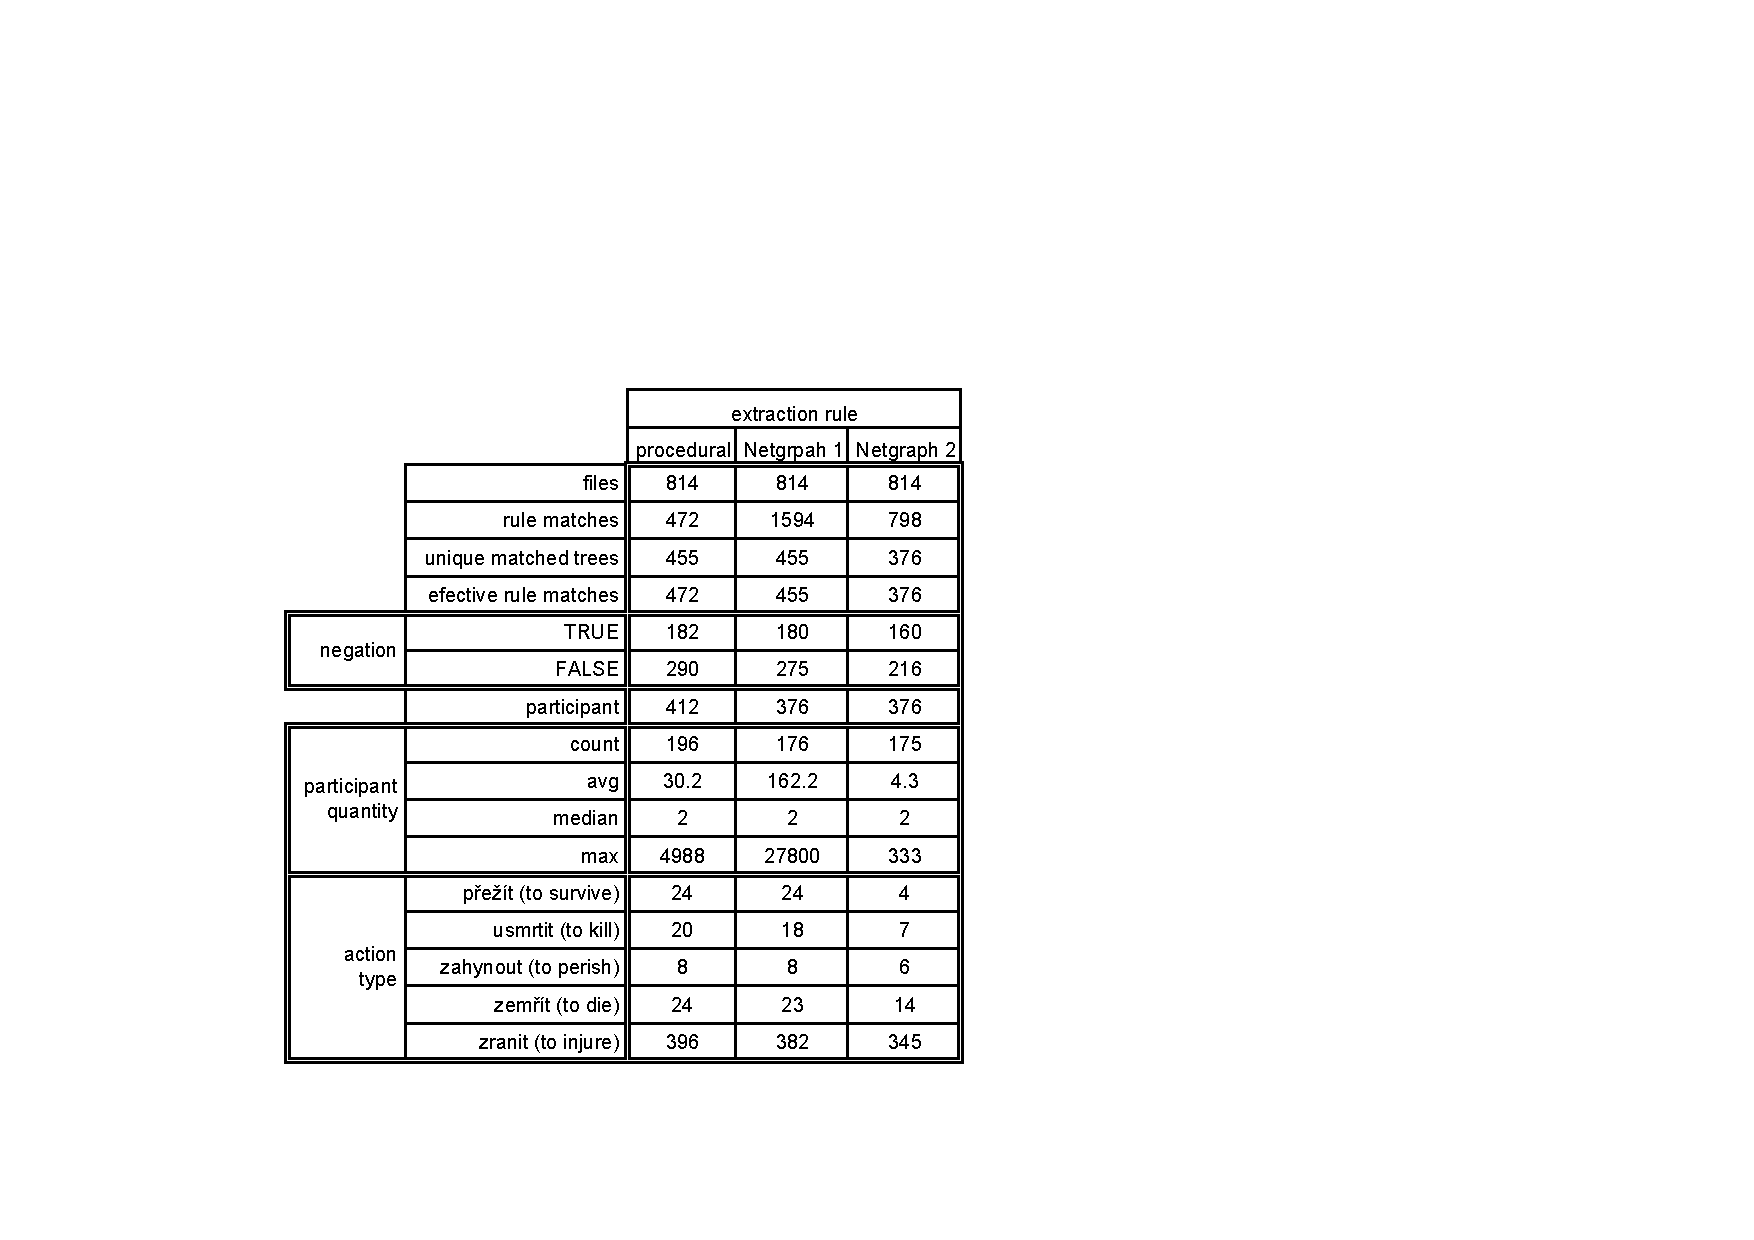
\includegraphics[angle=-90,width=0.6\hsize]{../img/ch3_tab_manual_rules}
	\caption{Evaluation of manually created rules (bigger dataset without manual annotations).}
	\label{tab:ch3_tab_manual_rules}
\end{table}



\begin{table}
	\centering
	\begin{tabular}{|r|c|c|c|c|c|c|}
		\hline
		 & correct & missing & spurious & recall & precision & F1\\
		\hline
		injuries & 3 & 29 & 0 & 0.09 & 1 & 0.17\\
		\hline
		fatalities & 1 & 10 & 0 & 0.09 & 1 & 0.17\\
		\hline
	\end{tabular}
	\caption{Evaluation of the manually created rule form Figure~\ref{fig:ch3_extract_patern} on the manually annotated dataset.}
	\label{tab:ch3_extract_patern_eval}
\end{table}



\begin{table}
	\centering
	\begin{tabular}{|r|c|c|c|c|c|c|}
		\hline
		 & correct & missing & spurious & recall & precision & F1\\
		\hline
		manual rules & 5 & 2 & 0 & 0.71 & 1 & 0.83\\
		\hline
		ILP rules & 5 & 2 & 0 & 0.71 & 1 & 0.83\\
		\hline
	\end{tabular}
	\caption{Evaluation of the manually created rules and ILP learned rules (manually annotated dataset was used for rule design (training half) and evaluation (testing half) -- see the description of the second experiment in text.)}
	\label{tab:ch3_damage_manual_eval}
\end{table}





\begin{table}
	\centering
	\begin{tabular}{|r|c|c|c|c|c|c|}
		\hline
		 & correct & missing & spurious & recall & precision & F1\\
		\hline
		manual rules & 4 & 1 & 1 & 0.8 & 0.8 & 0.8\\
		\hline
		ILP rules & 4 & 1 & 1 & 0.8 & 0.8 & 0.8\\
		\hline
	\end{tabular}
	\caption{Cross method comparison of found instances.}
	\label{tab:ch3_damage_cross_method}
\end{table}


